\section{Network Flows and Minimum Cost Flow algorithms}
\subsection{Totally unimodular matrices}
\begin{itemize}
	\item \textbf{Definition} En matrix $A$ er \textbf{totally modular}, hvis for en hver firkantet submatrix af $A$ har determinant $1$, $0$ eller $-1$  
  \item \textbf{Cramer's rule} Et system har en unik løsning hvis og kun hvis $\det(A) \neq 0$ og i det tilfælde er det givet ved
  \begin{equation*}
    x_i = \frac{\det{(A_i)}}{\det{A}}
  \end{equation*}
  hvor $A_i$ er $A$ hvor den søjle $i$ er erstatte med vektor $b$
  \item \textbf{Hoffman and Kruskal Theorem} $A=(a_{ij})$ være $m \times n$ matrix, så er $A$ unimodular hvis og kun hvis for enhver $b \in \mathbb Z^m$. Så er alle basic løsning af $F=\{Ax \leq b, x \geq 0\}$ integer
  \begin{proof} 
    Vi beviser kun, hvisretningen: Alle basic løsninger fås ved at introducere slack variablerne $x_{m+1}, \dots, x_{m+n}$ og vælge $n$ non-basic variabler til at sætte til 0 i systemet. System af variabler kan skrives i matrix form på følgende måde:
    \begin{equation*}
      [A \quad I] x = b
    \end{equation*}
    hvor $I$ er en $m \times m$ identitetsmatrice og $x \in \mathbb R^{n+m}$ består af både de originale variabler og slack variablerne. Dette kan løses unikt for de manglende $m$ basic variabler. Hvis vi fjerne alle nonbasic variabler fra systemet får vi følgende system
    \begin{equation*}
      \hat A \hat x = b
    \end{equation*}
    hvor $\hat A$ er $m \times m$ matricen kun indeholdende basic variaber og lad $\hat x$ være vektorene af basic variablerne. Ud fra Cramer's Rule har vi 
    \begin{equation*}
      \hat x_i = \frac{\det(\hat A_i)}{\det(\hat A)} \quad i=1,\dots,m
    \end{equation*}
    Siden $A$ og $b$ er integer må det betyde at $det(\hat A_i)$ også er integer. Da man kan udregne determinaten ved at gøre det efter rækker eller søjler skifter determinaten af submatricen af $A$ højest fortegn. Dermed bliver determinanten $\det(\hat A)$ enten $-1$ eller $1$ siden $A$ er en totally unimodular matrix. Dette medføre en derfor general integer løsninger. 

  \end{proof}
  \item Et lineært program er totally unimodular, hvis koefficient matrix $A$ er totally unimodular og $b$ har integer værdier
  \item \textbf{Lemma} Hvis $A$ er en matrix med elementer fra $\{-1,0,1\}$ med egenskaben at hver søjle indeholder mindst to ikke nul elementer, hvor højst en er $1$ og højest en er $-1$, så er $A$ totally unimodular
  \item \textbf{Lemma} Lad $A$ være en totally unimodular matrix
  \begin{itemize}
  	\item Så er $A^T$ totally unimodular
    \item Hvis man bytter om på søjler eller multiplier rækker eller søjler med $-1$, så er den resulterende matrix også totally unimodular
  \end{itemize} 
  \item \textbf{Lemma} Lad $A$ være totally unimodular, så er $[A \quad I]$ og $[A \quad A]$ totally unimodular
\end{itemize}

\subsection{Flow netværk}
\begin{itemize}
	\item Et \textbf{flow netværk} er en orienteret graf $D=(\mathcal N, \mathcal A)$
  \item Et \textbf{flow} er tildeling af værdier $x_{ij}>0$ for hver $ij \in \mathcal A$ 
  \item Et flow der overholder alle givne restrektioner for et given netværk kaldes et feasible flow
    \item \textbf{Balancen} af en knude $i$ er forskellen mellem det udgående flow og det indadgående flow:
    \begin{equation*}
      b_i(x) = \sum_{ij \in a} x_{ij} - \sum_{ji \in a} x_{ji}
    \end{equation*}
    \begin{itemize}
      \item Hvis en knude $i$ har $b_i(x) > 0$ kaldes $i$ for en \textbf{source} knude
      \item Hvis en knude $i$ har $b_i(x) > 0$ kaldes $i$ for en \textbf{sink} knude
      \item Hvis et flow hverken har source eller sink knuder kaldes det for en \textbf{circulation}
  \end{itemize}
  \item En \textbf{balance restrektioner} er specificeret af balancer $b_i$ for hver $i \in \mathcal N$ og siger at
  \begin{equation*}
 	  b_i(x) = b_i 
  \end{equation*}
  for alle $i \in \mathcal N$
  \begin{itemize}
  	\item Det er et krav at $\sum_{i \in \mathcal N} b_i = 0$ for at der eksisterer et feasible flow
  \end{itemize}
  \item \textbf{Arc restrektioner} er specificeret af \textbf{øvre grænser} $u_{ij}$ og nedre grænser $l_{ij}$ for alle $ij \in \mathcal A$ og kræver at
  \begin{equation*}
    l_{ij} \leq x_{ij} \leq u_{ij}
  \end{equation*}
  for alle $ij \in \mathcal A$ og det er et krav at $0 \leq l_{ij} \leq u_{ij}$ for alle $ij \in \mathcal A$ for at have feasible flows
\end{itemize}

\subsubsection{Minimum cost flow problem}
\begin{itemize}
	\item Minimum cost flow problemet er at minimere prisen af et given flow, som overholder en række restrektioner
  \item Alle kanter $ij \in \mathcal A$ har en pris $c_{ij}$, hvilket er prisen per unit der kommer igennem den givne kant
  \begin{itemize}
    \item Prisen kan også være et negativt nummer
    \item Prisen af et given flow er:
    \begin{equation*}
      c(x) = \sum_{ij \in \mathcal A} c_{ij}x_{ij} 
    \end{equation*}
  \end{itemize}
  \item Der bliver altid givet balance restrektioner
  \begin{itemize}
  	\item Kapacitets restrektioner er valgfri
  \end{itemize}
  \item \textbf{Integrality theorem} Lad $D=(\mathcal N, \mathcal A)$ være en netværk med cost $c_{ij} \in \mathcal R$, balance restrektioner $l_{ij}, u_{ij} \in \mathbb Z$ hvor $0 \leq l_{ij} \leq u_{ij}, \text{ for } ij \in \mathcal A$, så er der et minimum cost fesible flow $x$ med en integer værdi på hver kant \\
  \textbf{BEVIS?}
\end{itemize}

\subsubsection{Maximum $(s,t)$-flow problem}
\begin{itemize}
	\item I et $(s,t)$-flow problem et man givet et flow network $D=(\mathcal N, \mathcal A)$, sammen med to knuder $s,t \in \mathcal N$
  \begin{itemize}
  	\item Knuden $s$ er source knuden
  	\item Knuden $t$ er sink knuden
    \item \textbf{Flow conservation restrektionen} kræver at $b_i(x) = 0$ for alle $i \in \mathcal N \backslash \{s,t\}$
    \item Et flow er feasible hvis det opfylder
    \begin{itemize}
    	\item Ingen flows må være negative
      \item Flow conservation restrektionen
      \item De kant restrektioner givet ved øvre grænser
    \end{itemize}
    \item For et fesible flow defineres følgende som \textbf{værdi} $|x| = b_s(x)$
  \end{itemize}
  \item Et maximum $(s,t)$-flow problem med netværk $D=(\mathcal N, \mathcal A)$ med en specificeret source $s$ og sink $t$ kan laves om til et tilsvarende minimum flow problem med netværk $D'$ 
  \begin{itemize}
  	\item En ny kant fra $s$ til $t$ tilføjes til $D'$ med pris $-1$ og øvre grænse $\infty$
    \item Alle andre kanter har pris $0$
    \item Alle knuder har balance $+$
    \item Feasible flows $x$ i $D$ svarer til feasbile flows $x'$ i $D'$ hvor prisen af $x'$ er den negative værdi af $x$ 
  \end{itemize}
  \item Et $(s,t)$ snit af $D$ er en partition $(S,T)$ af knuderne af $D$ $\mathcal N = S \cup T$ således at $s \in S$ og $t \in T$ 
  \begin{itemize}
    \item \textbf{Kapaciteten} $u(S,T)$ af et $s(s,t)$ snit $(S,T)$ er følgende:
    \begin{equation*}
      u(S,T) = \sum_{\stackrel{ij \in \mathcal A}{i \in S, j \in T}} u_{ij}
    \end{equation*}
    \item \textbf{Minimumskapacitets $(s,t)$ snit problemet} er minimeringsproblem der finder det $(s,t)$ snit med mindst kapacitet
  \end{itemize}
  \item \textbf{Max-flow Min-flow Theorem}: Lad $x$ være et flow med maksimum værdi og lad $(S,T)$ være det $(s,t)$ snit med den mindste kapacitet, så gælder der:
  \begin{equation*}
    |x| = u(S,T)
  \end{equation*}
\end{itemize}

\subsection{Network simplex algoritme}
\begin{itemize}
	\item Det tilsvarende primal problem af et minimum cost problem er følgende:
  \begin{alignat*}{1}
    \text{min} \quad  & \sum_{ij \in \mathcal A} c_{ij}x_{ij} \\
    \text{s.t.} \quad & \sum_{ji \in \mathcal A} x_{ji} - \sum_{ij \in \mathcal A} x_{ij} = -b_i \\
    & x_{ij} \geq 0
  \end{alignat*}
	Dual problemet er følgende:
  \begin{alignat*}{1}
    \text{max} \quad  & -\sum_{i \in \mathcal N} b_i y_i \\
    \text{s.t.} \quad & y_j - y_i + z_{ij} = c_{ij} \quad ij \in \mathcal A \\
                      & z_{ij} \geq 0
  \end{alignat*}
  \item Et spanning tree og et balance flow som tildeler 0 til alle værdier ikke i spanning træet bliver kaldt en \textbf{træ løsning}
  \item Det er antaget af den givne network er connected
  \item \textbf{Theorem} En submatrix af $\mathcal A$ er en basis, hvis og kun hvis kanterne som svarer til søjler former et spanning træ
  \item Den duale variable $y_i$ svarer til kosten af forward kanter minus kosten af baglæns kanter
  \item Dual slack $z_{ij}$ for $ij \notin A$ svarer til prisen af forward kanterne minus prisen af backward kanterne i retning af cyklen formed af $i$ og $T$ i $ij$s retning
  \item \textbf{Initialisering:} 
  \begin{itemize}
    \item En basic løsning svarer til et spanning $T$ af netværket
    \item En rod $r$ bestemmes i $T$ 
    \item Primal løsning:
    \begin{itemize}
    	\item Sæt flow $0$ til kanter der ikke er i $T$ (non-basic variabler)
      \item Udregn flow på kanter i $T$ (basic variabler) ved at kører indad fra blade
    \end{itemize}
    \item Dual løsning:
    \begin{itemize}
    	\item Udregn dual variablerne (potential), ved at sætte $y_r = 0$ og løs $y_j = y_i + c_{ij}$ for alle $ij \in T$ og lad $z_{ij} = 0$
      \item Udregn de side dual slack $z_{ij}=c_{ij} - y_j +y_i$, for $ij \notin T$ 
    \end{itemize}
  \end{itemize}

  \item \textbf{Primal algoritme}
  \begin{itemize}
    \item Vælg en entering kant: Vælg en $ij \in \mathcal A$, hvor $z_{ij} < 0$
    \item Vælg en leaving kant: Givet cykel der kommer når man tilføjer den extra kant $ij$ og $T$ i retning af $ij$
    \begin{itemize}
    	\item Vælge en kant med modsatte retning med minimum flow vælrdi
      \item Send flow den retning for at udligne flow på denne edge
      \item Opdater dual løsning
    \end{itemize}
    \item Opdater dual løsning

  \end{itemize}
  \item \textbf{Dual algoritme}
  \begin{itemize}
    \item Vælg leaving kant: Vælg en arc $ij \in \mathcal T$ hvor $x_{ij} <0$ 
    \item Vælg en entering kan kant: Find en arc der sammen med $T$ laver en cycle i $ij$ retning
    \begin{itemize}
    	\item Vælg en sådan ark med minimum dual slack
      \item Send flow ad cyklen for at minimere flow på arc $ij$ til $0$ 
    \end{itemize}
    \item Opdatere dual løsning
  \end{itemize}
  \item Algoritmen stopper når $x$ og $(y,z)$ er feasible pga. strong duality theoremet:
  \begin{itemize}
  	\item Feasible løsninger $x$ og $(y,z)$ er begge optimale hvis og kun hvis $x_{ij}z_{ij} = 0$ for alle $ij \in \mathcal A$
  \end{itemize} 
  \item Den første basic solution kan findes vha. auxillary program eller vha. dual based fase 1
  \item For at sikre sig at algoritmen terminere skal anti-pivoting regler bruges
  \item Den er i værste tilfælde kører den i eksponentiel tid 
  \item Effektiv i praksis
\end{itemize} 

\subsection{Klein cycle cancelling algoritme}
\begin{lstlisting}[mathescape=true]
  Lad $x$ være et feasible flow.
  while exist
    $x:= x+ \gamma_C^{\delta(C)}$
  end while
  return $x$
\end{lstlisting}
\begin{itemize}
	\item Den kigger på en netværk $D= (\mathcal N, \mathcal A)$ med balancer $b_i$, nedre grænser $l_{ij}$, øvre grænse $u_{ij}$ og priser $c_{ij}$
  \item Denne algoritme begrænser sig ikke til træ løsninger, men lader enhver cykel i netværket være en kandat til at gøre løsningen bedre
  \item Lad $C$ være en cykel i $D$ 
  \begin{itemize}
  	\item Lad $F$ være mængden af forward kanter i $C$
    \item Lad $B$ være mængden af backward kanter i $C$
    \item Prisen for en given cykel $C$ er defineret, som:
    \begin{equation*}
      c(C) = \sum_{ij \in F} c_{ij} - \sum_{ij\in B} c_{ij}
    \end{equation*}
  \end{itemize}
  \item Given et nummer $\delta$, definere cykel flow $\gamma_C^\delta$ som
  \begin{equation*}
    \gamma_C^\delta =
      \begin{cases}
        \mbox{$\delta$} & \mbox{if $ij \in F$} \\
        \mbox{$-\delta$} & \mbox{if $ij \in B$} \\
        \mbox{$0$} & \mbox{otherwise} 
      \end{cases}
  \end{equation*}
  \item Givet en cykel $C$ i $D$ gælder følgende
  \begin{enumerate}
  	\item Flowet $\gamma_C^\delta$ er en cirkulation dvs. $b_i(\gamma_C^\delta) = 0$ for alle $i \in \mathcal N$
	  \item Prisen af $\gamma_C^\delta$ er $c(\gamma_C^\delta) = \delta \cdot c(C)$
  \end{enumerate}
  \item Lad $x$ være et feasible flow i $D$ og lad $C$ være en cykel i $D$. Så er $C$ en 
\textbf{augmenting cykel} relativ til $x$, hvis $c(C)<0$ og der eksister et $\delta > 0$ således at $x+\gamma_C^\delta$ er et feasible flow i $D$
  \begin{itemize}
    \item Når $C$ er en cykel med $c(C)<0$. Så er $C$ en augumenting cykel relativ til $x$ hvis og kun hvis $x_{ij} < u_{ij}$ for alle $ij \in F$ og $l_{ij} < x_{ij}$ for alle $ij \in B$.
    \item For at finde den maksimale værdi $\delta$ for en augumenting cycle, hvor $x + \gamma_C^\delta$ stadig er et feasible flow findes $\delta(C)$ på følgende måde
    \begin{equation*}
      \delta(C) = \min \bigg\{\min_{ij \in F}(u_{ij}-x_{ij}), \min_{ij \in B}(x_{ij}-l_{ij})\bigg\}
    \end{equation*}
  \end{itemize} 
  \begin{figure}[h]
    \centering
    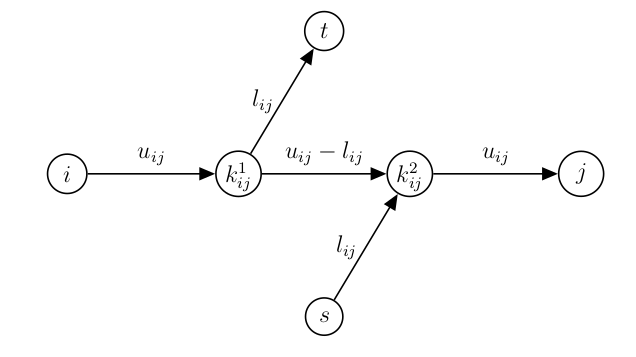
\includegraphics[width=260px]{img/edge_feasible}
    \caption{Den del af $D'$ der svarer to kanten $ij$ fra $D$ \label{edge-flow}}
  \end{figure}
  \item For at finde et feasible flow til grafen formuleres det som et maksimum flow problem, hvor man givet et flow netværk $D=(\mathcal N, \mathcal A)$ bygges et nyt flow netværk $D' = (\mathcal N', \mathcal A')$
  \begin{itemize}
  	\item Dette problem kan løses af Ford-Fulkerson eller Edmonds-Karp algoritmen
		\item $\mathcal N' = \{s,t\} \cup \mathcal N \cup \{k_{ij}^\ell \mid ij \in \mathcal A, \ell = 1,2\}$
    \item Kanterne i $D'$ der svarer til kanterne $ij \in \mathcal A$ er som beskrevet på Figur \ref{edge-flow}
    \item Fra $s$ har vi kanter til hver $i \in \mathcal N$ hvor $b_i > 0$ med øvre grænse $b_i$ 
    \item Til $t$ har vi kanter til hver $i \in \mathcal N$ hvor $b_i < 0$ med øvre grænse $-b_i$ 
    \item $D$ har et feasible flow, hvis og kun hvis $D'$ har et $(s,t)$ flow $x'$, hvor alle kanter fra source $s$ er fulde 
  \end{itemize}
  \item For at finde en argumenting cycle i en graf $D=(\mathcal N, \mathcal A)$ med nedre grænser $l_{ij}$, øvre grænser $u_{ij}$ og pris $c_{ij}$ defineres et residual netværk $D_x= (\mathcal N, \mathcal A_x)$ relativ til det nuværende flow $x$
  \begin{itemize}
  	\item Kanterne af $D_x$ indikerer hvor meget man kan ændre flowet af $x$ samtidig med at man overholder feasibility
    \item Kanterne $A_x$ af $D_x$ er følgende:
    \begin{equation*}
      \mathcal A_x = \{ij \mid ij \in \mathcal A \land x_{ij} < u_{ij} \} \cup \{ji \mid \ij \in \mathcal A \land \l_{ij} < x_{ij} \}
    \end{equation*}
    \item Når $x_{ij} < u_{ij}$ gives kanten $ij \in A_x$ den øvre grænse $(u_x)_{ij} = u_{ij} - x_{ij}$ og prisen $(c_x)_{ij} = c_{ij}$
	  \item Når $l_{ij} < x_{ij}$ gives kanten $ji \in \mathcal A_x$ den øvre grænse $(u_x)_{ji} = x_{ij} - l_{ij}$ og prisen $(c_x)_{ji} = -c_{ij}$
    \item Balancen af alle knuder er sat til $0$ 
    \item Alle knuder af $D_x$ har nedre grænse $0$ 
    \item Problemet med at finde et feasible flow i $D$ relativ til $x$ er præcist problemet med at finde negative vægtet cykler i $D_x$, når man bruger prisen som vægte. 
    \begin{itemize}
    	\item Bellman Ford eller Floyd Warshall kan bruges til dette
    \end{itemize}
  \end{itemize}
  \item \textbf{Circulation Decomposition Lemma}. Lad $x$ være en ikke negativ circulation flow i et netværk $D=(\mathcal N, \mathcal A)$. Så eksister der cykler $C_1, \dots, C_k$ og  tal $\delta_1, \dots, \delta,k \geq 0$ så ledes at
  \begin{equation*}
    x = \gamma_{C_1}^{\delta_1} + \gamma_{C_2}^{\delta_2} + \dots + \gamma_{C_k}^{\delta_k}
  \end{equation*}

  \item \textbf{Lemma} Lad $D$ være et netværk med et feaasible flow $x$. Hvis $x$ ikke er en minimum kost flow, så eksister der en augumenting cykel
  \item Siden prisen bliver bedre hver iteration, garanterer dette at algoritmen stopper  
  \item Den kører i værste tilfælde eksponentiel mange gange
\end{itemize}
% \subsubsection{Find en argumenting cykel}
% \subsubsection{Correctness}

\newpage
%%% Local Variables:
%%% mode: latex
%%% TeX-master: "optimering-noter"
%%% End:
